% !TeX root = lfgw.tex
\chapter{Prüfungen aufsetzen: exam}

exam\footcite{ziegenhagen:dtk2016/2}



\section{Einleitung}

CTAN hält eine Reihe von Paketen bereit, um Klausuren und Übungsblätter zu setzen, neben \texttt{exam} sind hier \texttt{eqexam}, \texttt{exercise} und \texttt{exsheets} zu nennen. Im folgenden möchte ich nur auf \texttt{exam} weiter eingehen, dem geneigten Leser sei die Lektüre der Dokumentationen für die anderen Pakete ans Herz gelegt.

\texttt{exam} wird von Philip Hirschhorn (Wellesley College, USA) betreut, das Paket kann auf eine Geschichte zurückblicken, die bis ins Jahr 1994 reicht. Die aktuelle Version, die als Grundlage für diesen Artikel dient, datiert auf Mai 2015. Da mein Artikel nicht alle Funktionen der Klasse detailliert beschreiben kann, erlaube man mir schon an dieser Stelle einen Hinweis auf die exzellente Dokumentation, die auf mehr als 100 Seiten den Umgang mit \texttt{exam} erläutert.

\section{Minimalbeispiel}

Listing \ref{lis:b01} zeigt ein Minimalbeispiel, das eine einzelne Frage in ein Dokument setzt. Neben der obligatorischen Angabe der Dokumentenklasse \texttt{exam}, die intern auf \texttt{article} basiert, werden alle Fragen mittels \texttt{\textbackslash question} Befehl in eine \texttt{questions} Umgebung gesetzt. 

\begin{lstlisting}[caption={Minimalbeispiel \texttt{beispiel-01.tex}},label={lis:b01}]
\documentclass[12pt]{exam}
\begin{document}
\begin{questions}
\question[5]
Wieviel wiegt Luft?

\question[5]
Wieviel wiegt Blei?
\end{questions}
\end{document}
\end{lstlisting}

Dem  \texttt{\textbackslash question} Befehl kann noch optional die Anzahl der möglichen Punkte für diese Frage übergeben werden. \texttt{exam} kann -- sofern die Klassenoption \enquote{addpoints} gesetzt ist -- die Punkte zusammenaddieren und auch eine Bewertungstabelle ausgeben; eine hilfreiche Funktion, die den Dozenten vor lästigen Rechenfehlern bewahren kann.

Neben \enquote{addpoints} gibt es noch eine weitere Klassenoption, die an dieser Stelle nicht unerwähnt bleiben soll: \enquote{answers}. Sie steuert, ob die Antworten auf eine Frage unter die Frage gesetzt werden sollen oder nicht, dazu später mehr.

Betrachten wir uns das Ergebnis von \ref{lis:b01} in Abbildung \ref{fig:b01}, so fällt auf dass statt \enquote{Punkte} \enquote{points} gesetzt wurde. Dies liegt daran, dass das Paket standardmäßig mit englischen Begriffen arbeitet, die erst eingedeutscht werden müssen. Außerdem war das Minimalbeispiel so minimal, dass eine Reihe von nützlichen oder notwendigen Paketen noch nicht eingebunden ist. Da ich persönlich noch am liebsten mit \texttt{pdflatex} arbeite, enthält meine Paketliste (siehe Listing \ref{lis:pak}) noch Pakete, die bei der Nutzung von xe\LaTeX\ oder lua\LaTeX\ nicht unbedingt notwendig sind.

\begin{figure}
\fbox{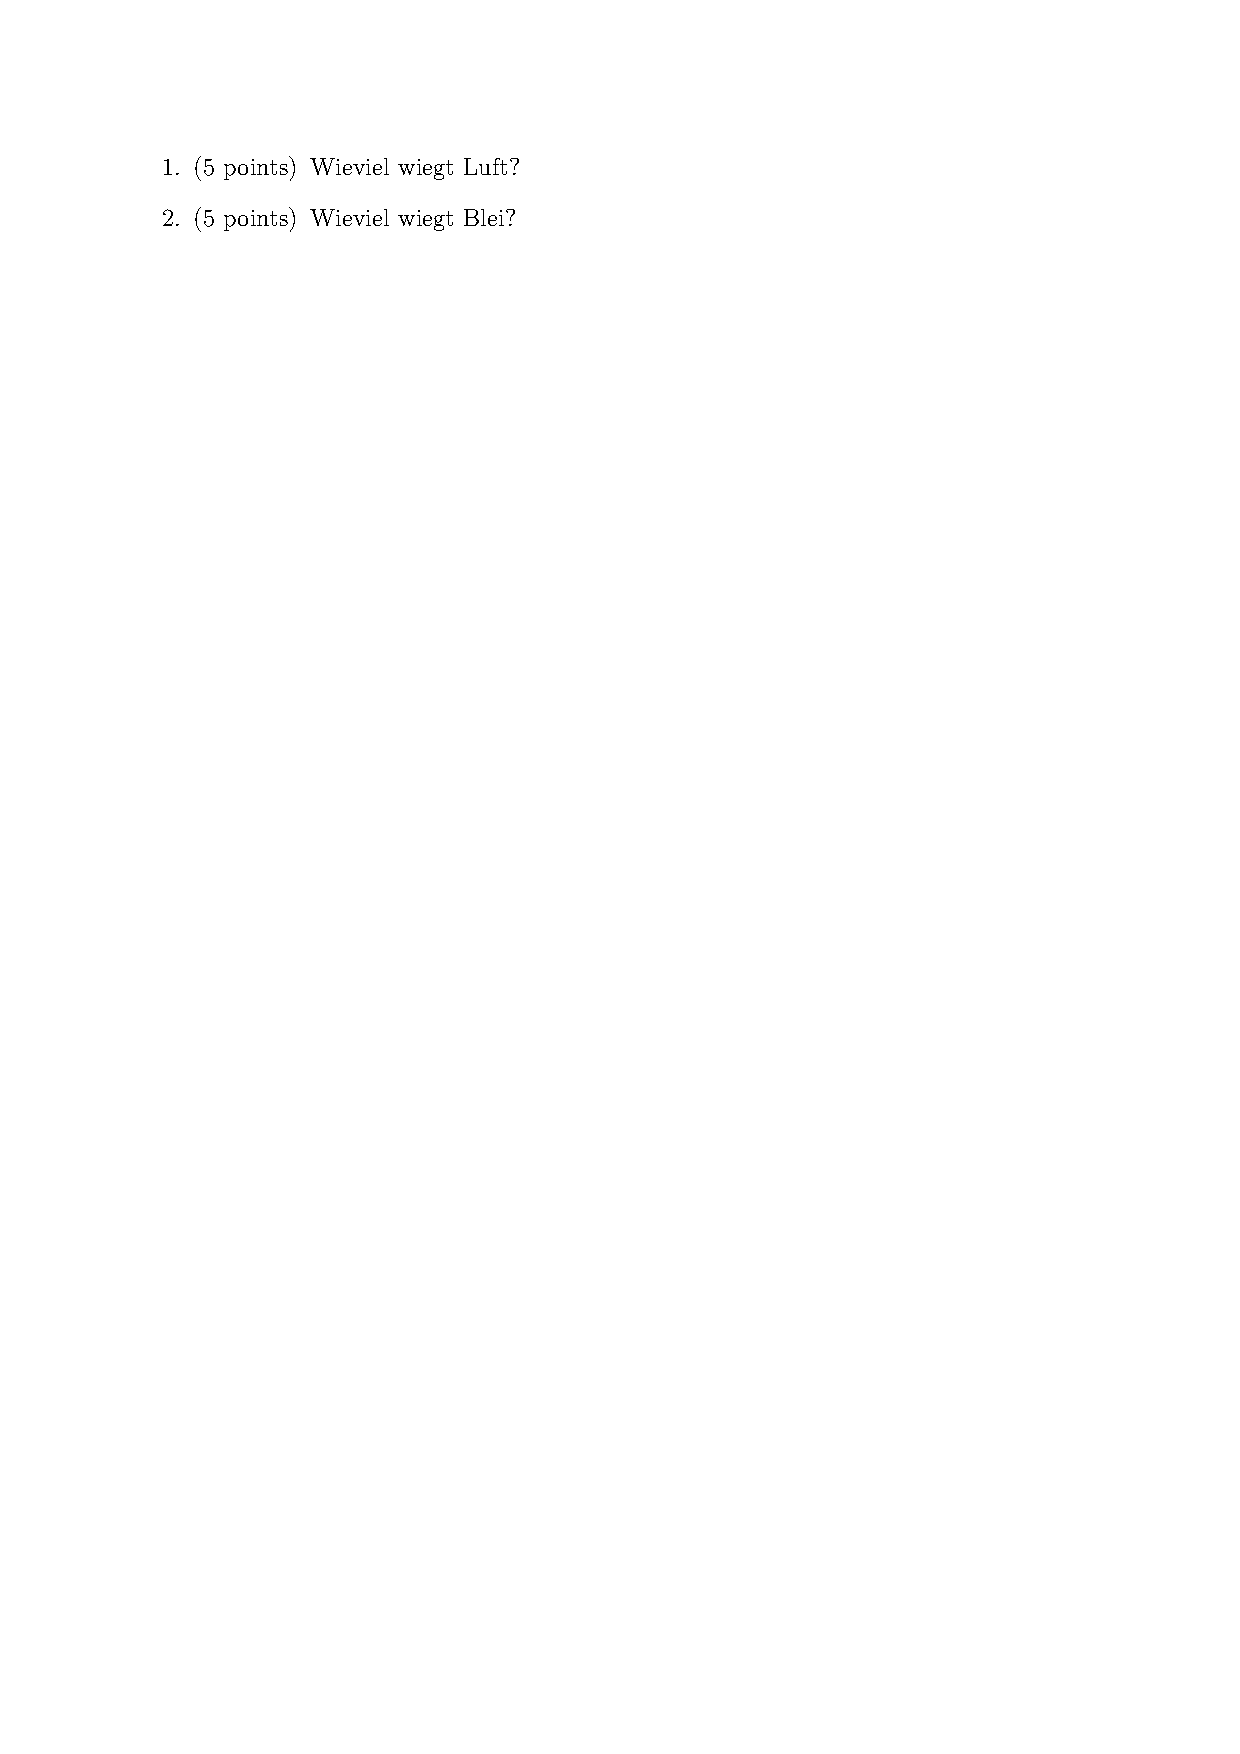
\includegraphics[clip,trim=2cm 25cm 6cm 1cm,width=\textwidth]{./Examples/exam/beispiel-01}}
\caption{Ergebnis von Listing \ref{lis:b01}, \texttt{beispiel-01.tex}}\label{fig:b01}
\end{figure}

\begin{lstlisting}[label={lis:pak},caption={Paketliste (pdf\LaTeX)}]
\usepackage[ngerman]{babel} % ngerman mal nicht als Klassenoption
\usepackage[utf8]{inputenc}
\usepackage[T1]{fontenc}
\usepackage{booktabs} % schöne Tabellen
\usepackage{csquotes} % Anführungszeichen mit \enquote{}
\usepackage{paralist} % für kompakte Aufzählungen
\usepackage[math]{iwona} % Font mit Mathe-Support
\usepackage{amsmath,textcomp,tikz} %diverses
\usepackage{eso-pic} % Bilder im Hintergrund
\end{lstlisting}

Die Anpassung der Begriffe geschieht in \texttt{exam} über spezielle Befehle, eine Auswahl der in späteren Beispielen notwendigen finden sich in Listing \ref{lis:lang}, die Dokumentation enthält noch eine Reihe anderer entsprechender Befehle.

\begin{lstlisting}[label={lis:lang},caption={Eindeutschung der Fachbegriffe}]
\pointpoints{Punkt}{Punkte}
\bonuspointpoints{Bonuspunkt}{Bonuspunkte}
\renewcommand{\solutiontitle}{\noindent\textbf{Lösung:}\enspace}
 
\chqword{Frage}   
\chpgword{Seite} 
\chpword{Punkte}   
\chbpword{Bonus Punkte} 
\chsword{Erreicht}   
\chtword{Gesamt}

\hpword{Punkte:} % Punktetabelle
\hsword{Ergebnis:}
\hqword{Aufgabe:}
\htword{Summe:}
\end{lstlisting}

Kombinieren wir nun die Paketliste aus Listing \ref{lis:pak} mit dem Minimalbeispiel aus Listing \ref{lis:b01}, so erhalten wir beim Übersetzen die Ausgabe von Abbildung \ref{fig:b02}.

\begin{figure}[b]
\fbox{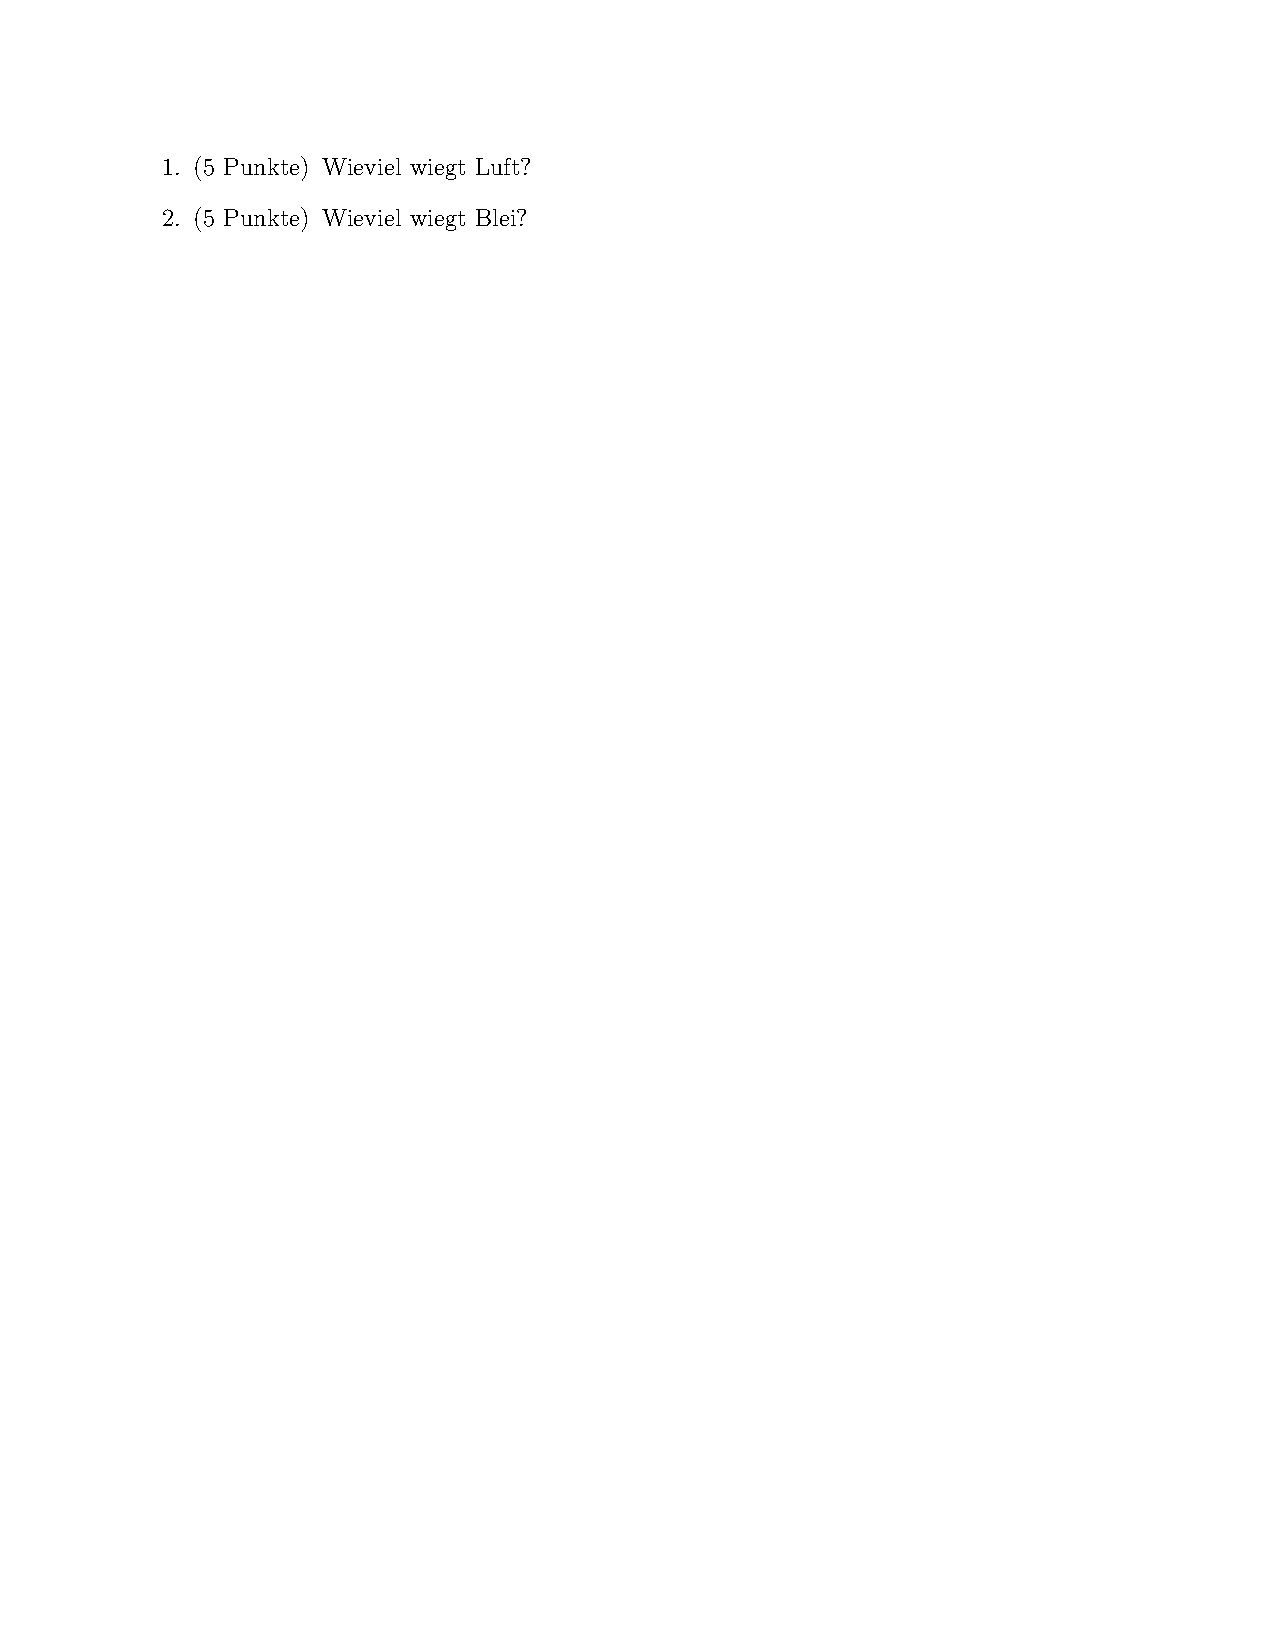
\includegraphics[clip,trim=1cm 22cm 8cm 1cm,width=\textwidth]{./Examples/exam/beispiel-02}}
\caption{Listings \ref{lis:b01} und \ref{lis:lang} kombiniert, \texttt{beispiel-02.tex}}\label{fig:b02}
\end{figure}

\section{Formatierung von Kopf \& Fuß}

\texttt{exam} bietet eine Reihe von Möglichkeiten für die Anpassung von Kopf und Fuß. Listing \ref{lis:headfoot} zeigt, wie \texttt{firstpageheader} und -\texttt{footer} für die Titelseite beziehungsweise \texttt{runningpageheader} und -\texttt{footer} für Folgeseiten mit Angabe von Fach und Dozent ausgestattet werden können. Horizontale Linien unter den Kopfzeilen werden durch die entsprechenden \texttt{\dots headrule} Befehle gesetzt. Abbildung \ref{fig:headfoot} zeigt das entsprechende Ergebnis.

\begin{lstlisting}[caption={Definition von Kopf und Fuß auf Titel- und Folgeseiten},label={lis:headfoot}]
\newcommand{\dozent}{Dr. Uwe Ziegenhagen}
\newcommand{\fach}{Klausur Statistik}
 
\pagestyle{headandfoot}
\firstpageheadrule
\runningheadrule

\firstpageheader{}{}{\dozent \\ \fach}
\runningheader{}{}{\dozent \\ \fach}
\firstpagefooter{}{}{\thepage\,/\,\numpages}
\runningfooter{}{}{\thepage\,/\,\numpages}
\end{lstlisting}


\begin{figure}[b]
\fbox{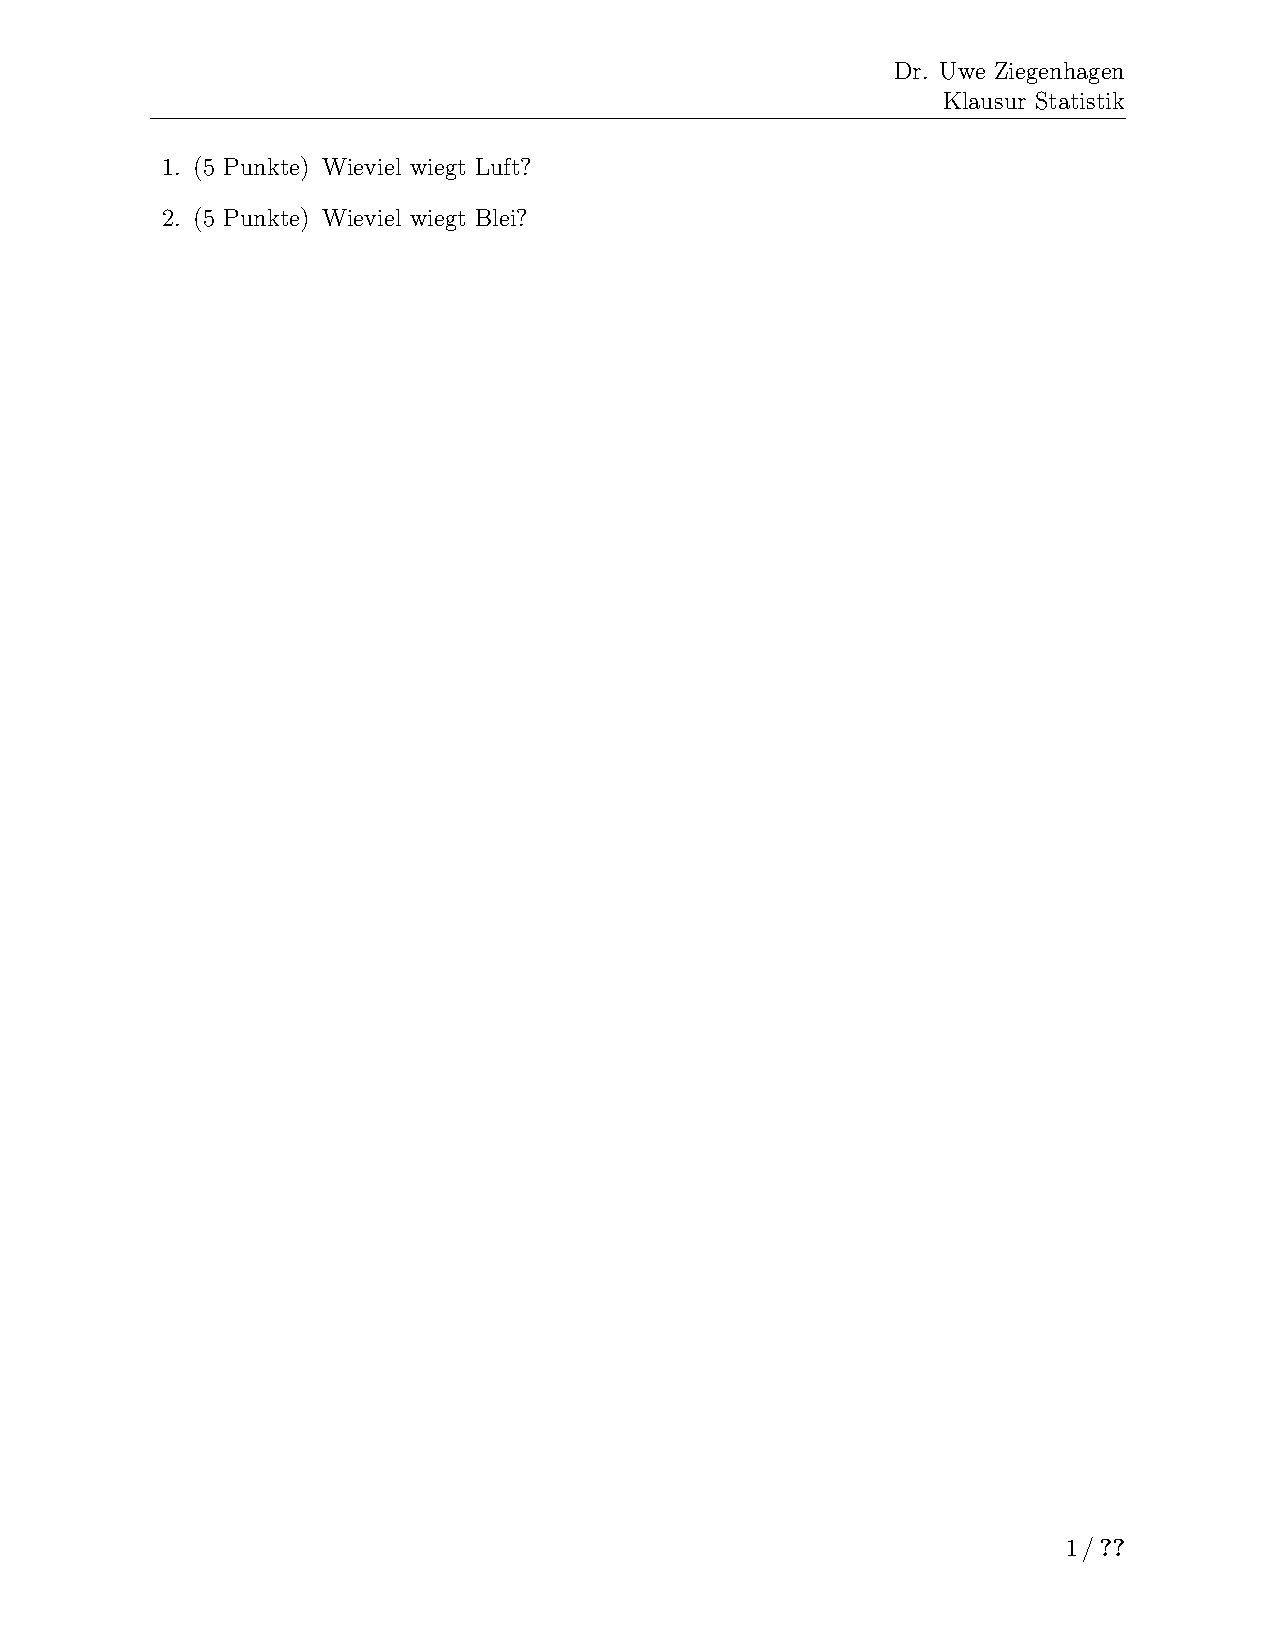
\includegraphics[trim=2cm 18cm 2cm 0.5cm,width=\textwidth]{./Examples/exam/beispiel-03}}
\caption{Ergebnis von Listing \ref{lis:headfoot}, \texttt{beispiel-03.tex}}\label{fig:headfoot}
\end{figure}

\clearpage

\section{Einfügen von Teilfragen}

Einzelne Fragen, die mit \texttt{\textbackslash question} gesetzt wurden, lassen sich noch in Unterfragen unterteilen. \texttt{exam} bietet dazu folgende Umgebungen und dazugehörige Befehle an, die wie \texttt{\textbackslash question} zu nutzen sind:

\begin{itemize}
	\item \texttt{parts} Umgebung mit \texttt{\textbackslash part} Befehl
	\item \texttt{subparts} Umgebung mit \texttt{\textbackslash subpart} Befehl
	\item \texttt{subsubparts} Umgebung mit \texttt{\textbackslash subsubpart} Befehl
\end{itemize}

Listing \ref{lis:parts} zeigt, wie man eine Frage in zwei \texttt{\textbackslash part} Unterfragen unterteilt, Abbildung \ref{fig:allparts} die Ausgabe eines erweiterten Beispiels, das auch \texttt{\textbackslash subpart} und \texttt{\textbackslash subsubpart} nutzt.

\begin{lstlisting}[caption={Beispiel für die Nutzung von \texttt{parts} und \texttt{\textbackslash part}}, label={lis:parts}]
\question[5]
Wieviel wiegt Luft?

\begin{parts}
\part[3] Geben Sie den Wert in Gramm pro Kubikmeter an!

\part[2] Geben Sie den Wert in Kilogramm pro Kubikkilometer an!
\end{parts}
\end{lstlisting}


\begin{figure}[b]
\fbox{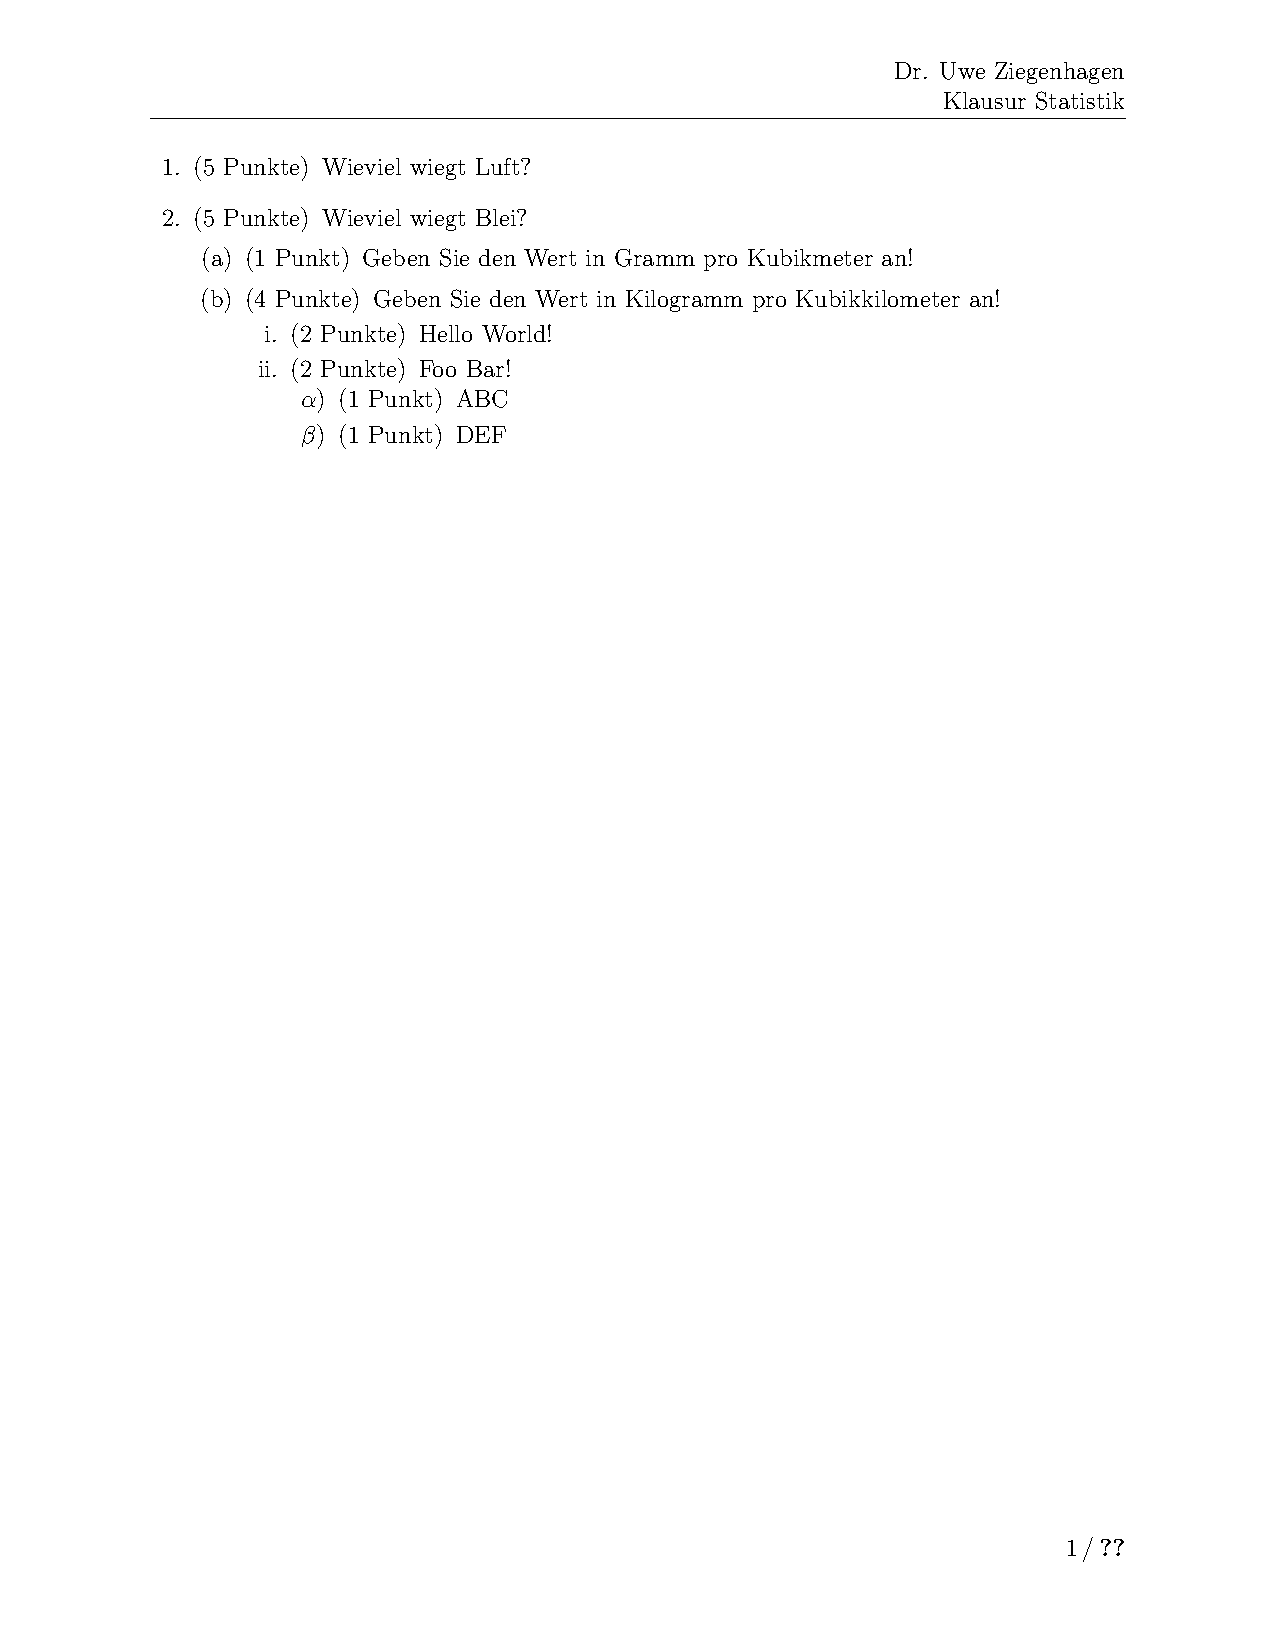
\includegraphics[trim=2cm 19cm 2cm 0.5cm,width=\textwidth]{./Examples/exam/beispiel-04}}
\caption{Ergebnis von Listing \ref{lis:parts}, \texttt{beispiel-04.tex}}\label{fig:allparts}
\end{figure}


\section{Weitere Aufgabentypen}

Neben Textaufgaben unterstützt \texttt{exam} auch sogenannte Multiple-Choice Aufgaben und Lückentexte. 
Es stellt dazu folgende Umgebungen bzw. Befehle bereit:

\begin{description}
\item[choices] Umgebung, stellt dem Eintrag einen Buchstaben voran
\item[checkboxes] Umgebung, nutzt keinen Buchstaben sondern einen  Kreis, der angekreuzt werden kann
\item[oneparcheckboxes] Umgebung wie \texttt{checkboxes}, jedoch in einem Absatz nebeneinander anstatt untereinander
\item[fillin] Befehl für Lückentext, als optionaler Parameter wird das Lösungswort übergeben
\end{description}

Für die drei genannten Umgebungen gilt, dass die jeweils richtige Antwort bzw. die richtigen Antworten mittels \texttt{\textbackslash CorrectChoice} von den falschen Antworten unterschieden werden können. Setzt man die \enquote{answers} Option wie oben beschrieben als Klassenoption, so werden diese richtigen Antworten entsprechend markiert. Listing \ref{lis:mchoice1} und \ref{lis:mchoice2} zeigen die entsprechenden Code-Beispiele, Abbildung \ref{fig:mchoicea} die Ausgabe mit \enquote{answers} aktiviert.

\begin{lstlisting}[caption={Multiple-Choice Aufgaben 1},label={lis:mchoice1}]
\question Wer war kein Beatle?

\begin{choices}
\choice John
\choice Paul
\choice George
\choice Ringo
\CorrectChoice Socrates
\end{choices}

\question Wer war kein Beatle?

\begin{checkboxes}
\choice John
\choice Paul
\choice George
\choice Ringo
\CorrectChoice Socrates
\end{checkboxes}
\end{lstlisting}

\clearpage

\begin{lstlisting}[caption={Multiple-Choice Aufgaben 2},label={lis:mchoice2}]

\question Wer war kein Beatle?

\begin{oneparcheckboxes}
\choice John
\choice Paul
\choice George
\choice Ringo
\CorrectChoice Socrates
\end{oneparcheckboxes}

\question \fillin[James Bond] ist der coolste Superheld.

\end{lstlisting}

\begin{figure}
\fbox{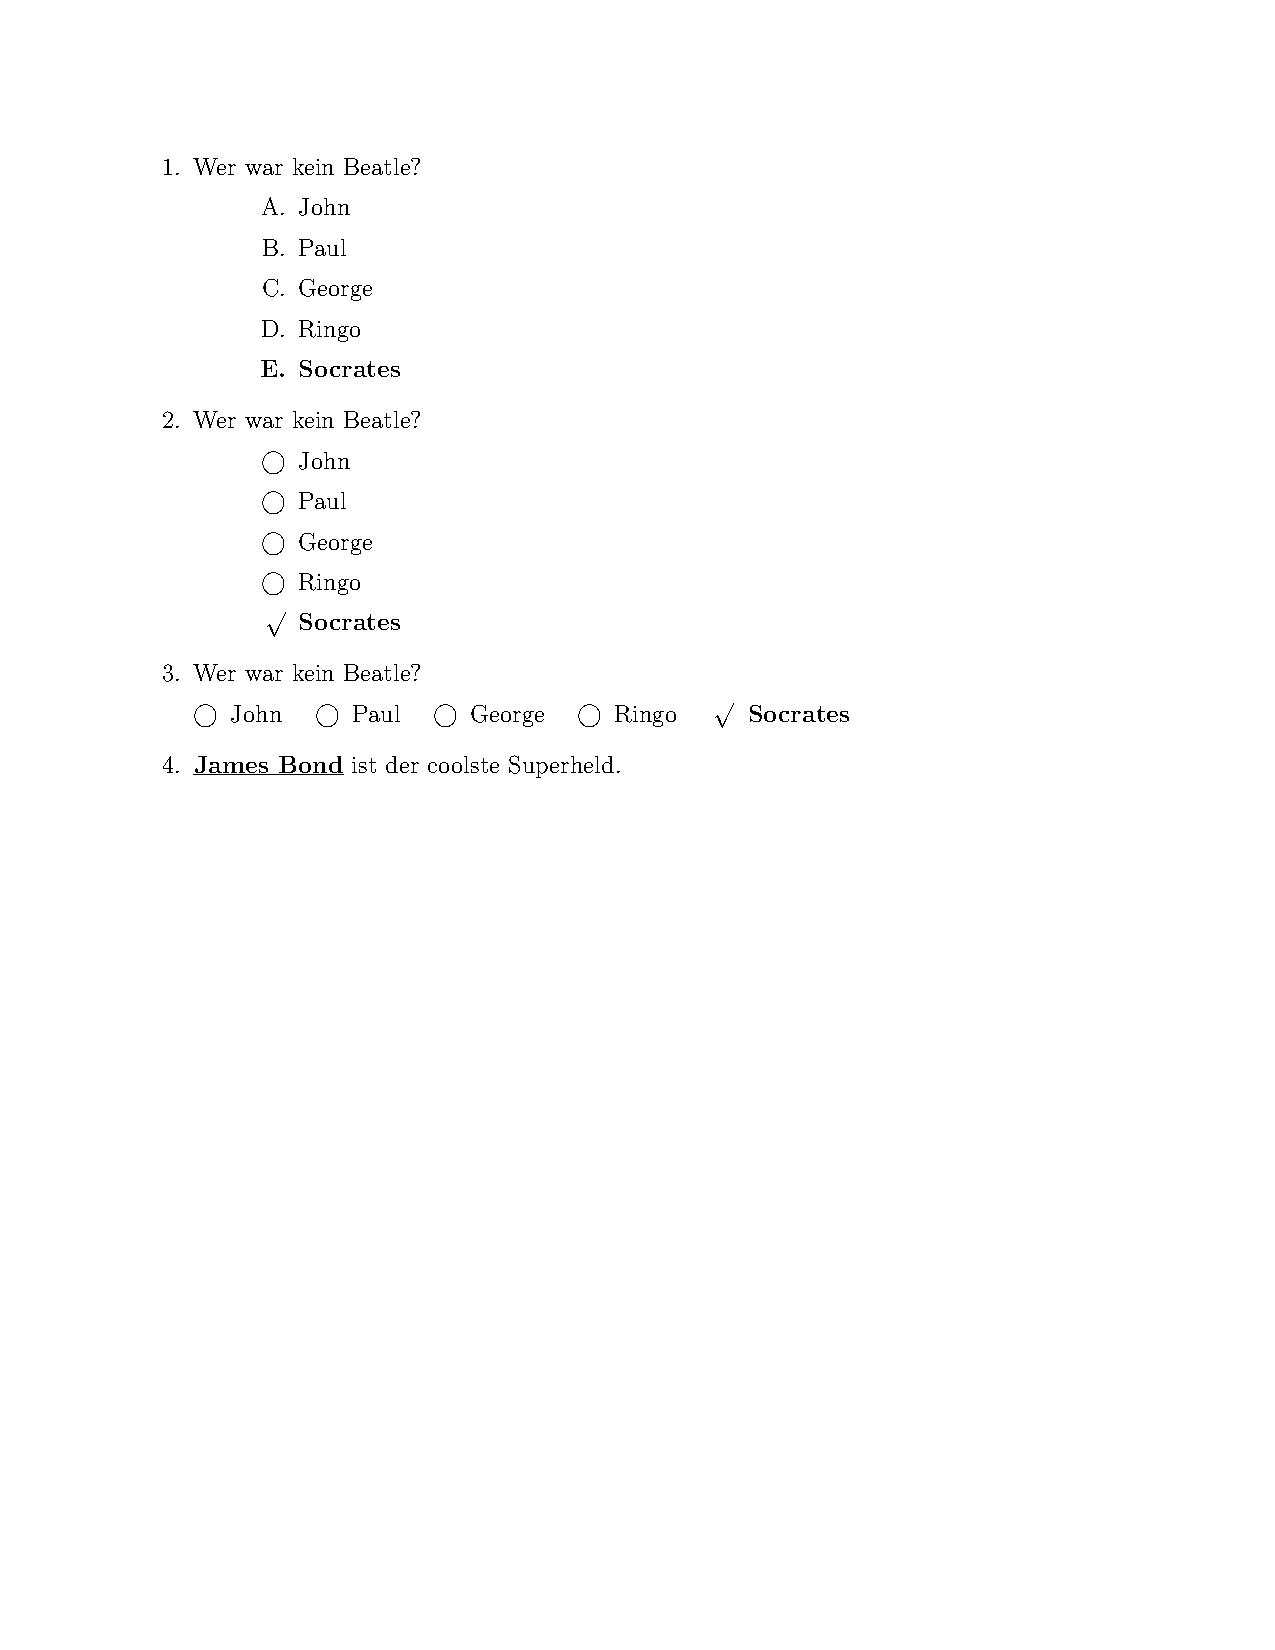
\includegraphics[trim=1cm 13.5cm 3cm 1cm,width=0.95\textwidth]{./Examples/exam/beispiel-06}}
\caption{Listings \ref{lis:mchoice1} und \ref{lis:mchoice2} kombiniert, \texttt{beispiel-06.tex}}\label{fig:mchoicea}
\end{figure}

\clearpage

\section{Platz für Antworten}

\texttt{exam} erlaubt es dem Dozenten auch, unterschiedliche Leerräume für die Antworten von Schülern und Studenten bereitzuhalten. Neben einfachem Leerraum mittels \texttt{\textbackslash vspace} und umrahmten Boxen mittels (siehe Listing \ref{lis:vspace1} sowie die Ausgabe in Abbildung \ref{fig:vspace1}) stellt \texttt{exam} auch linierte und gepunktete Linien sowie karierten Platz bereit.

\begin{lstlisting}[caption={Leerraum und Boxen für Antworten}, label={lis:vspace1}]
% einfacher Abstand
\vspace{<Länge>}

%bis zum Seitenende
\vspace*{\stretch{1}}
\newpage

% leere umrahmte Box
\makeemptybox{<Länge>}

%leere umrahmte Box bis zum Seitenende
\makeemptybox{\stretch{1}}
\newpage
\end{lstlisting}

\begin{figure}[b]
\fbox{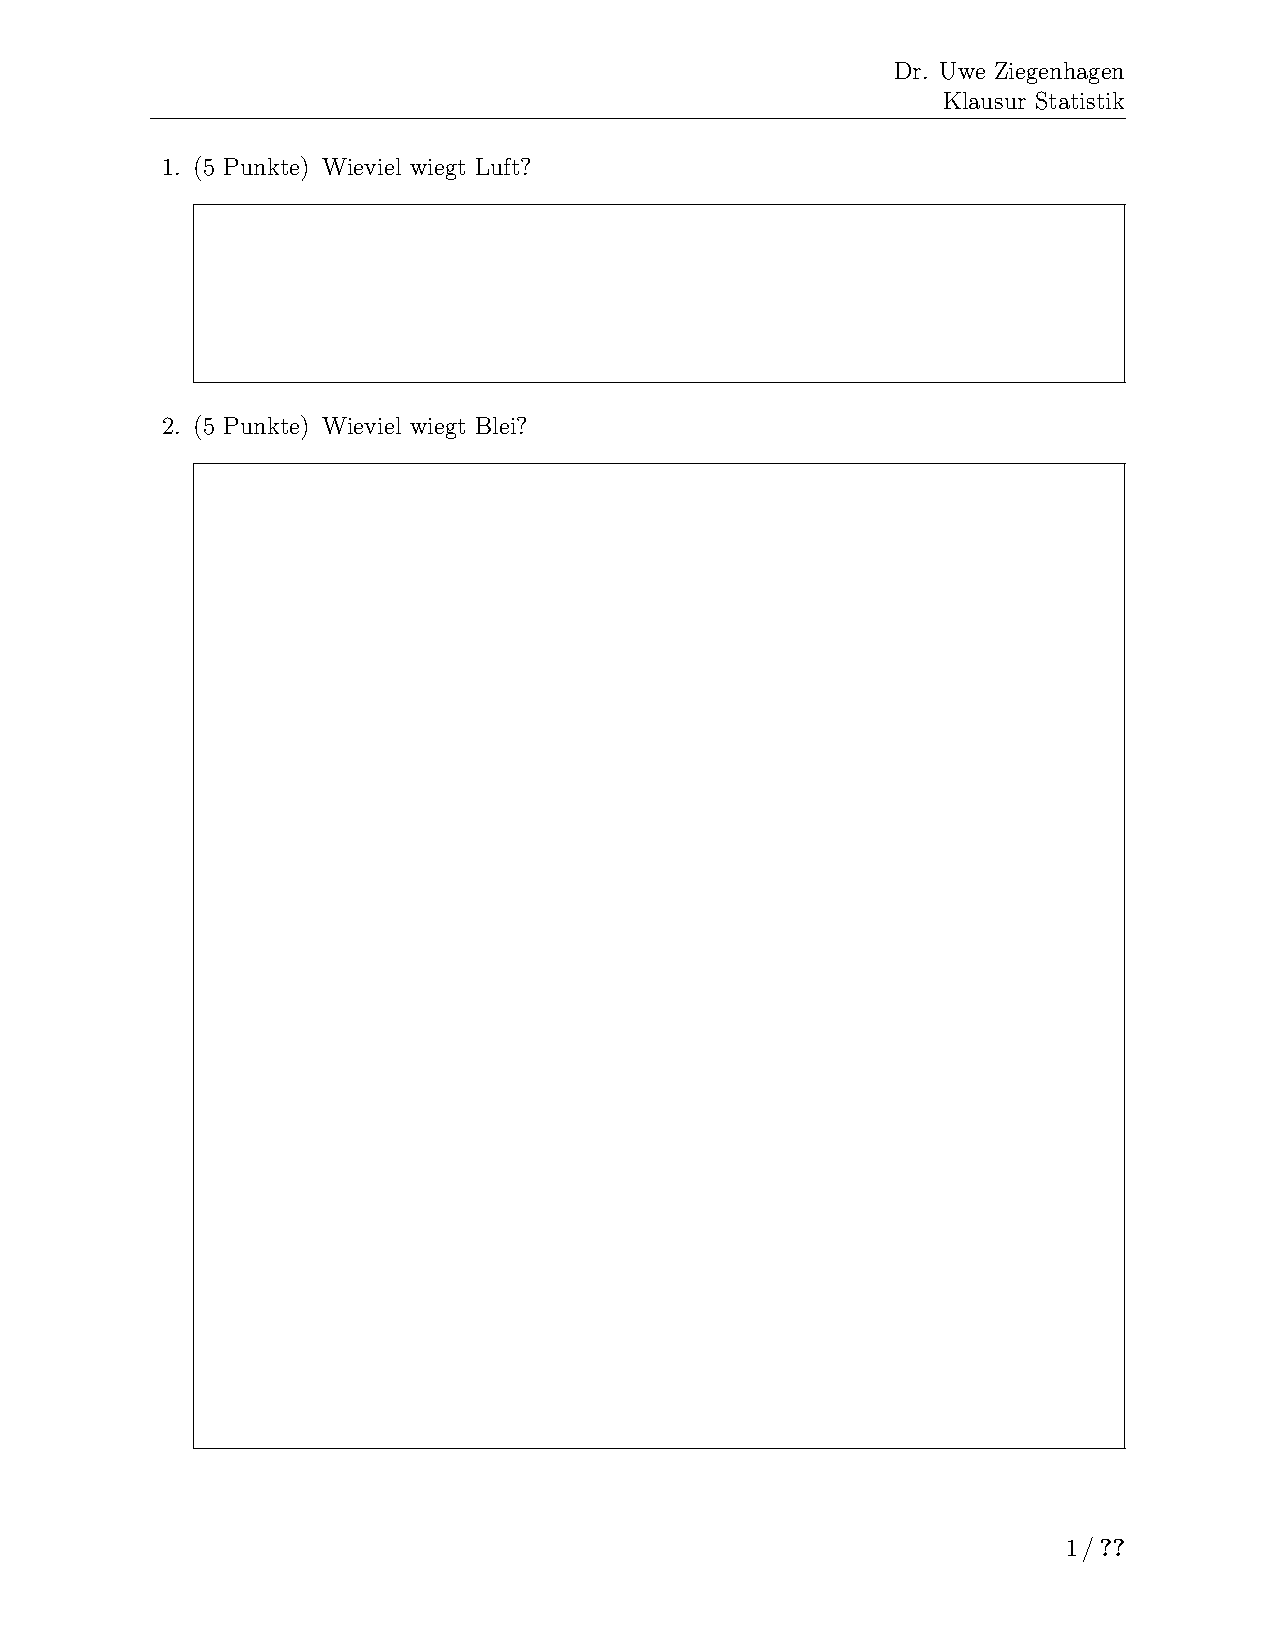
\includegraphics[clip, trim=2cm 17cm 1.5cm 2.5cm,width=\textwidth]{./Examples/exam/beispiel-07}} % 
\caption{Ergebnis von Listing \ref{lis:vspace1}, \texttt{beispiel-07.tex}}\label{fig:vspace1}
\end{figure}

Für Linien nutzt man \texttt{\textbackslash fillwithlines}, für gepunktete Linien \texttt{\textbackslash fillwithdottedlines}, und für ein kariertes Raster \texttt{\textbackslash fillwithgrid}. Alle drei Befehle benötigen als Parameter die vertikale Länge des Platzes, den sie für die Antworten reservieren sollen. Außerdem stellt \texttt{exam} noch den \texttt{\textbackslash answerline} Befehl bereit, der Platz für ein Wort oder einen Satz schafft, der optional für die Lösungsausgabe angegeben werden kann.

Beispiele für die Nutzung dieser Befehle finden sich in Listing \ref{lis:fill}, für die Ausgaben siehe die Abbildungen \ref{fig:fill1} und \ref{fig:fill2}. 

\begin{lstlisting}[caption={Beispiele für Linien und Gitter},label={lis:fill}]
\fillwithlines{<Länge>} % für linierten Platz
% Hinweis: \linefillheight für Abstand zwischen Linien

\fillwithdottedlines{<Länge>} % für gepunktete Linien
% Hinweis: Abstand in \dottedlinefillheight

\fillwithgrid{<Länge>} % 
% \setlength{\gridsize}{5mm}
% \setlength{\gridlinewidth}{0.1pt}

\answerline[Antwort] % für kurze Antworten
\end{lstlisting}

\begin{figure}[b]
\fbox{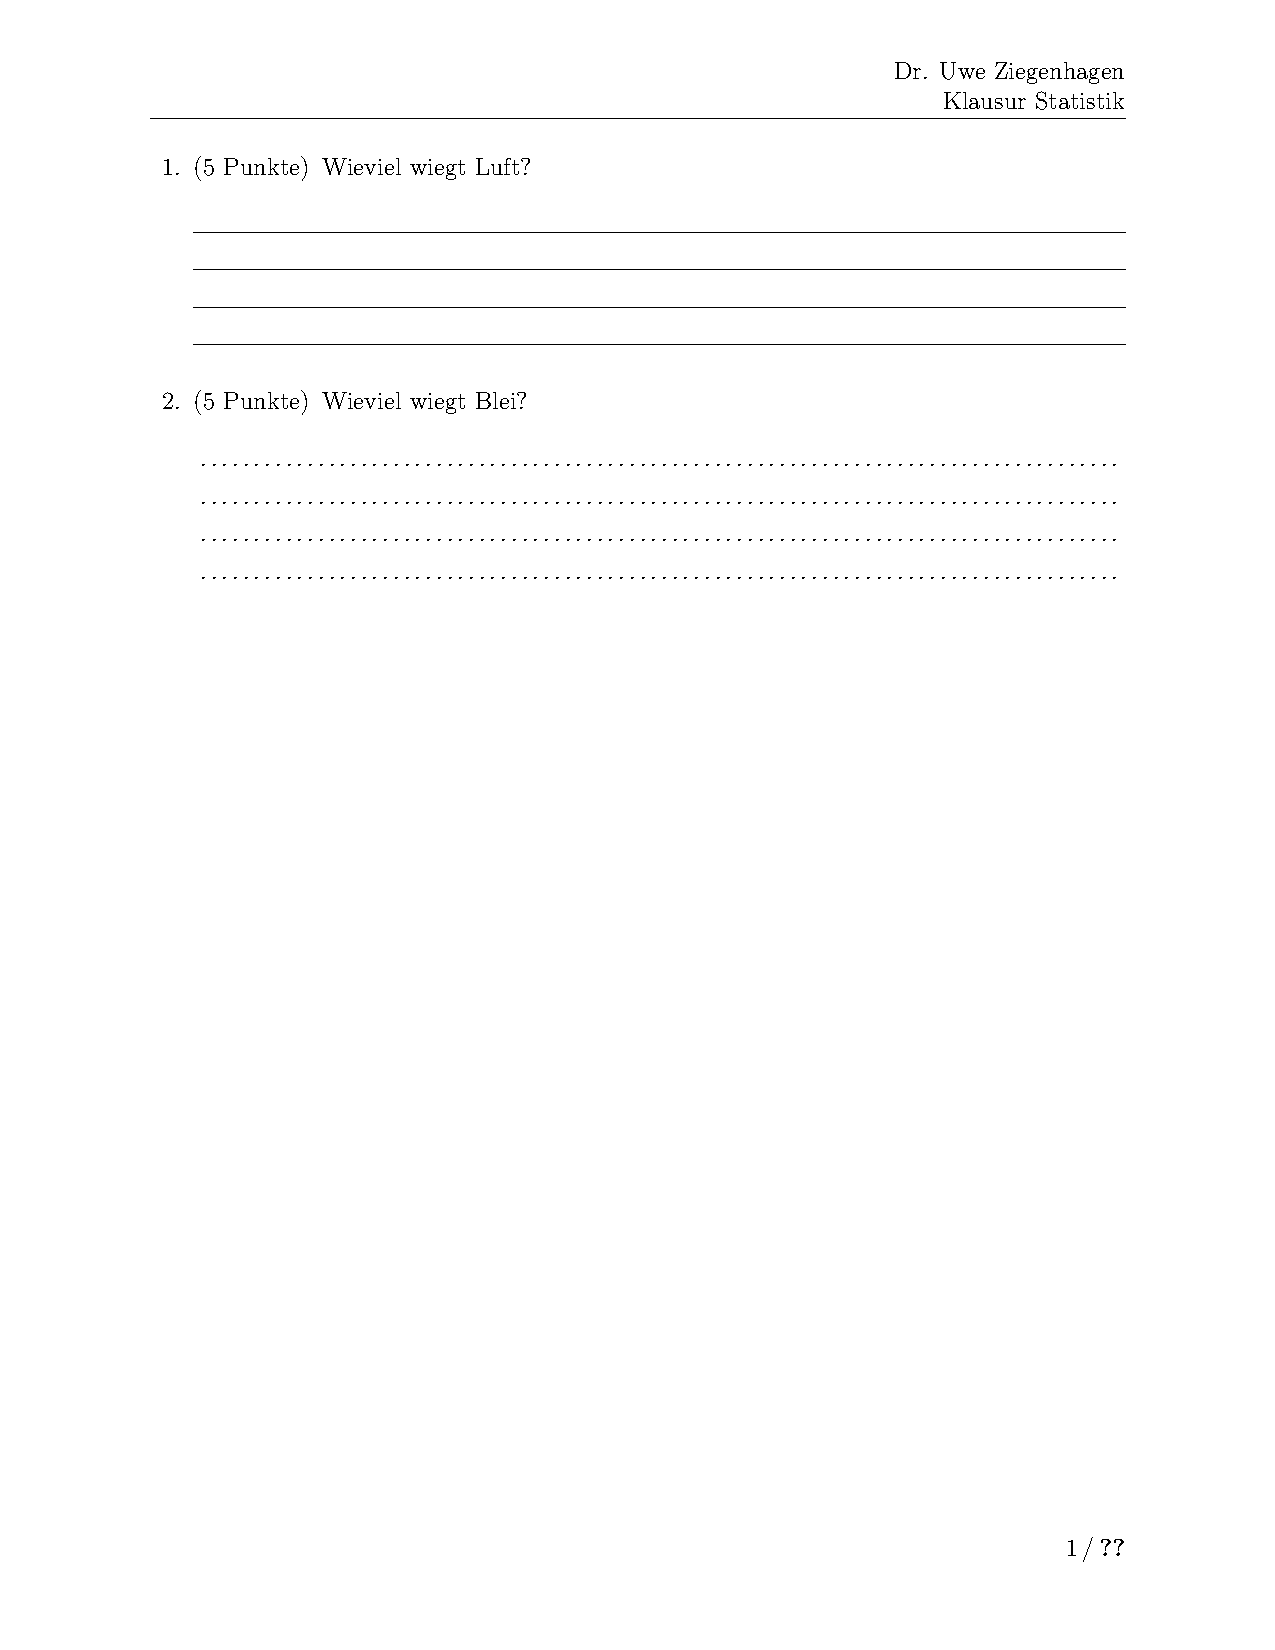
\includegraphics[clip, trim=2cm 16.5cm 2cm 2.5cm,width=\textwidth]{./Examples/exam/beispiel-08}} % 
\caption{Ausgabe von Listing \ref{lis:fill}, Teil 1}\label{fig:fill1}
\end{figure}

\begin{figure}
\fbox{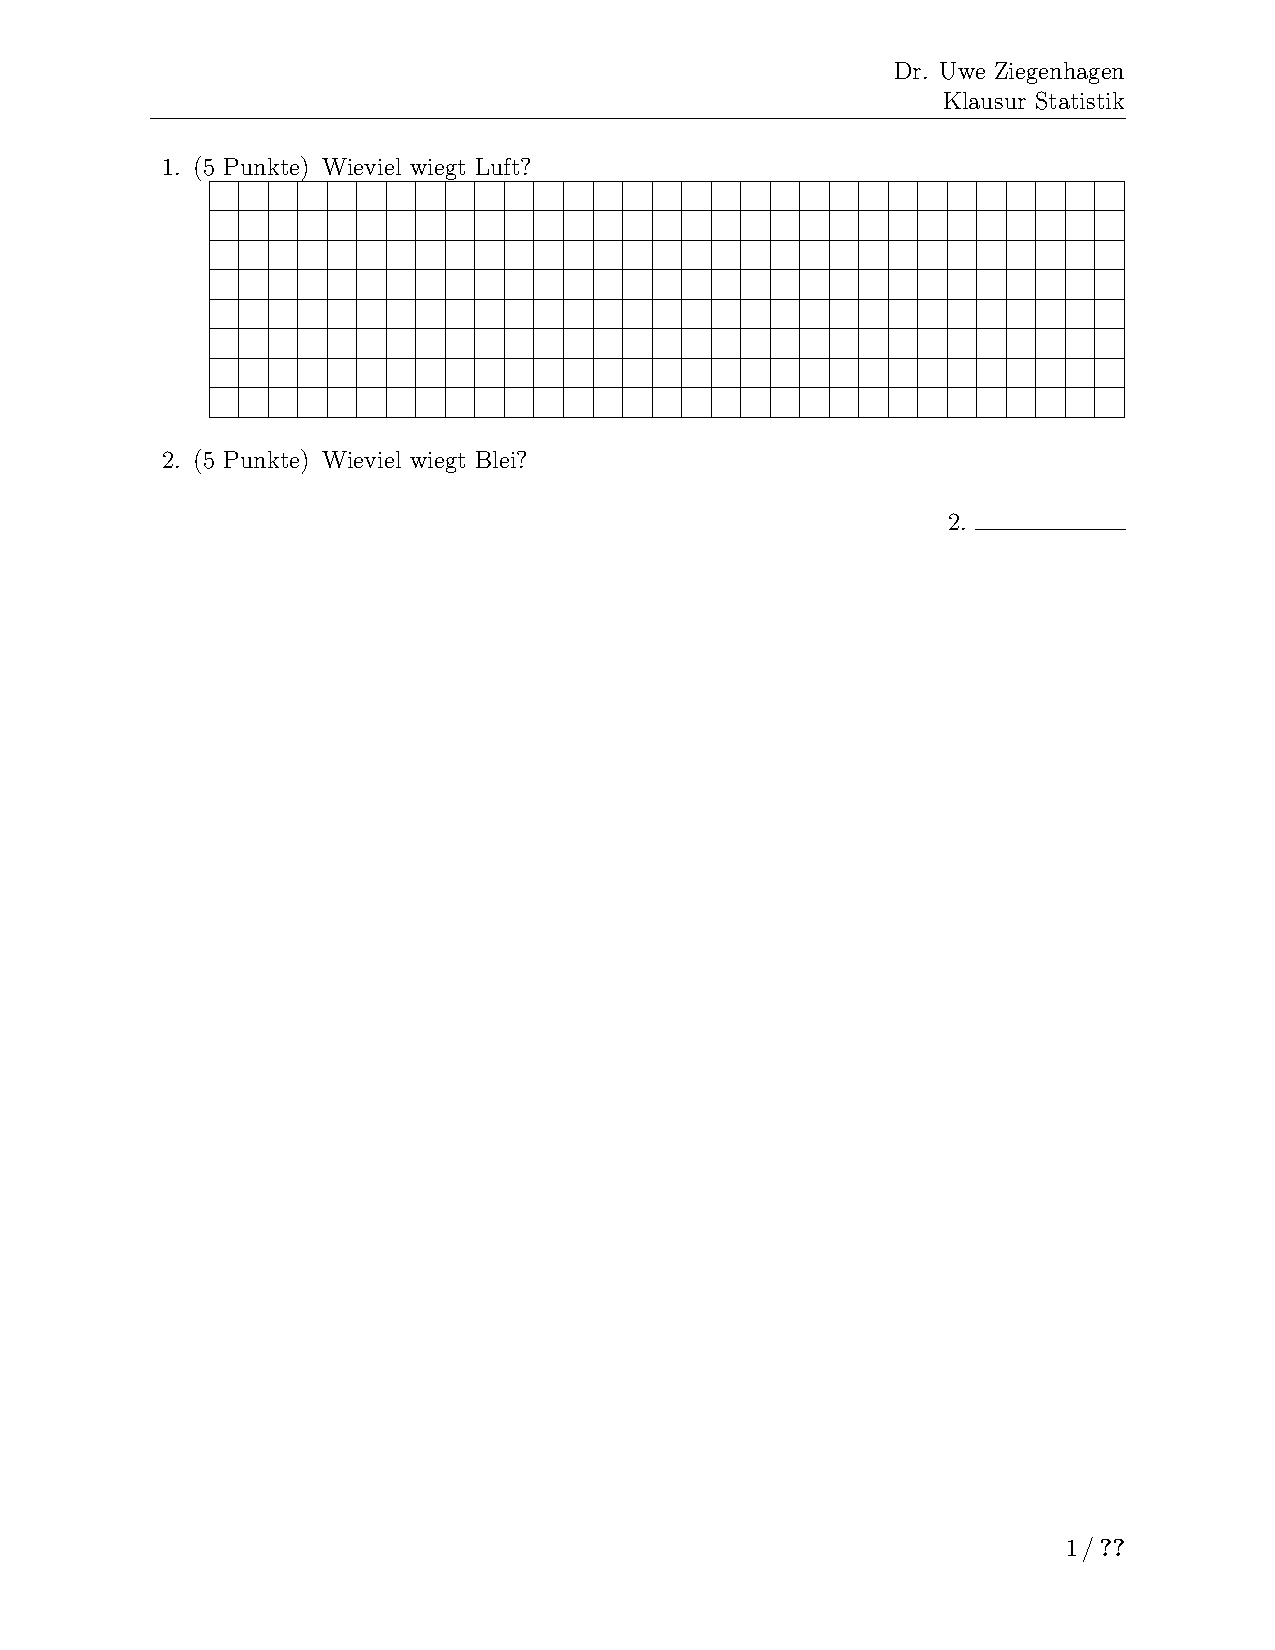
\includegraphics[clip, trim=2cm 18cm 2cm 2.5cm,width=\textwidth]{./Examples/exam/beispiel-09}} % 
\caption{Ausgabe von Listing \ref{lis:fill}, Teil 2}\label{fig:fill2}
\end{figure}

\section{Ausgabe von Lösungen}

Wie bereits erwähnt, steuert die globale Option \enquote{answers}, ob die hinterlegten Lösungen angezeigt werden sollen oder nicht. Die Hinterlegung von Lösungen bei Textaufgaben im Text erfolgt dabei über eingefügte \texttt{solution} Umgebungen, die hinter jede \texttt{\textbackslash question} gesetzt werden, Listing \ref{lis:sol1} zeigt ein entsprechendes Beispiel, Abbildung \ref{fig:sol2} die entsprechende Ausgabe.

\begin{lstlisting}[label={lis:sol1},caption={Beispielhafte Lösung}]
\question Was ist die Antwort auf alle Fragen?

\begin{solution}
42
\end{solution}
\end{lstlisting}

\begin{figure}
\fbox{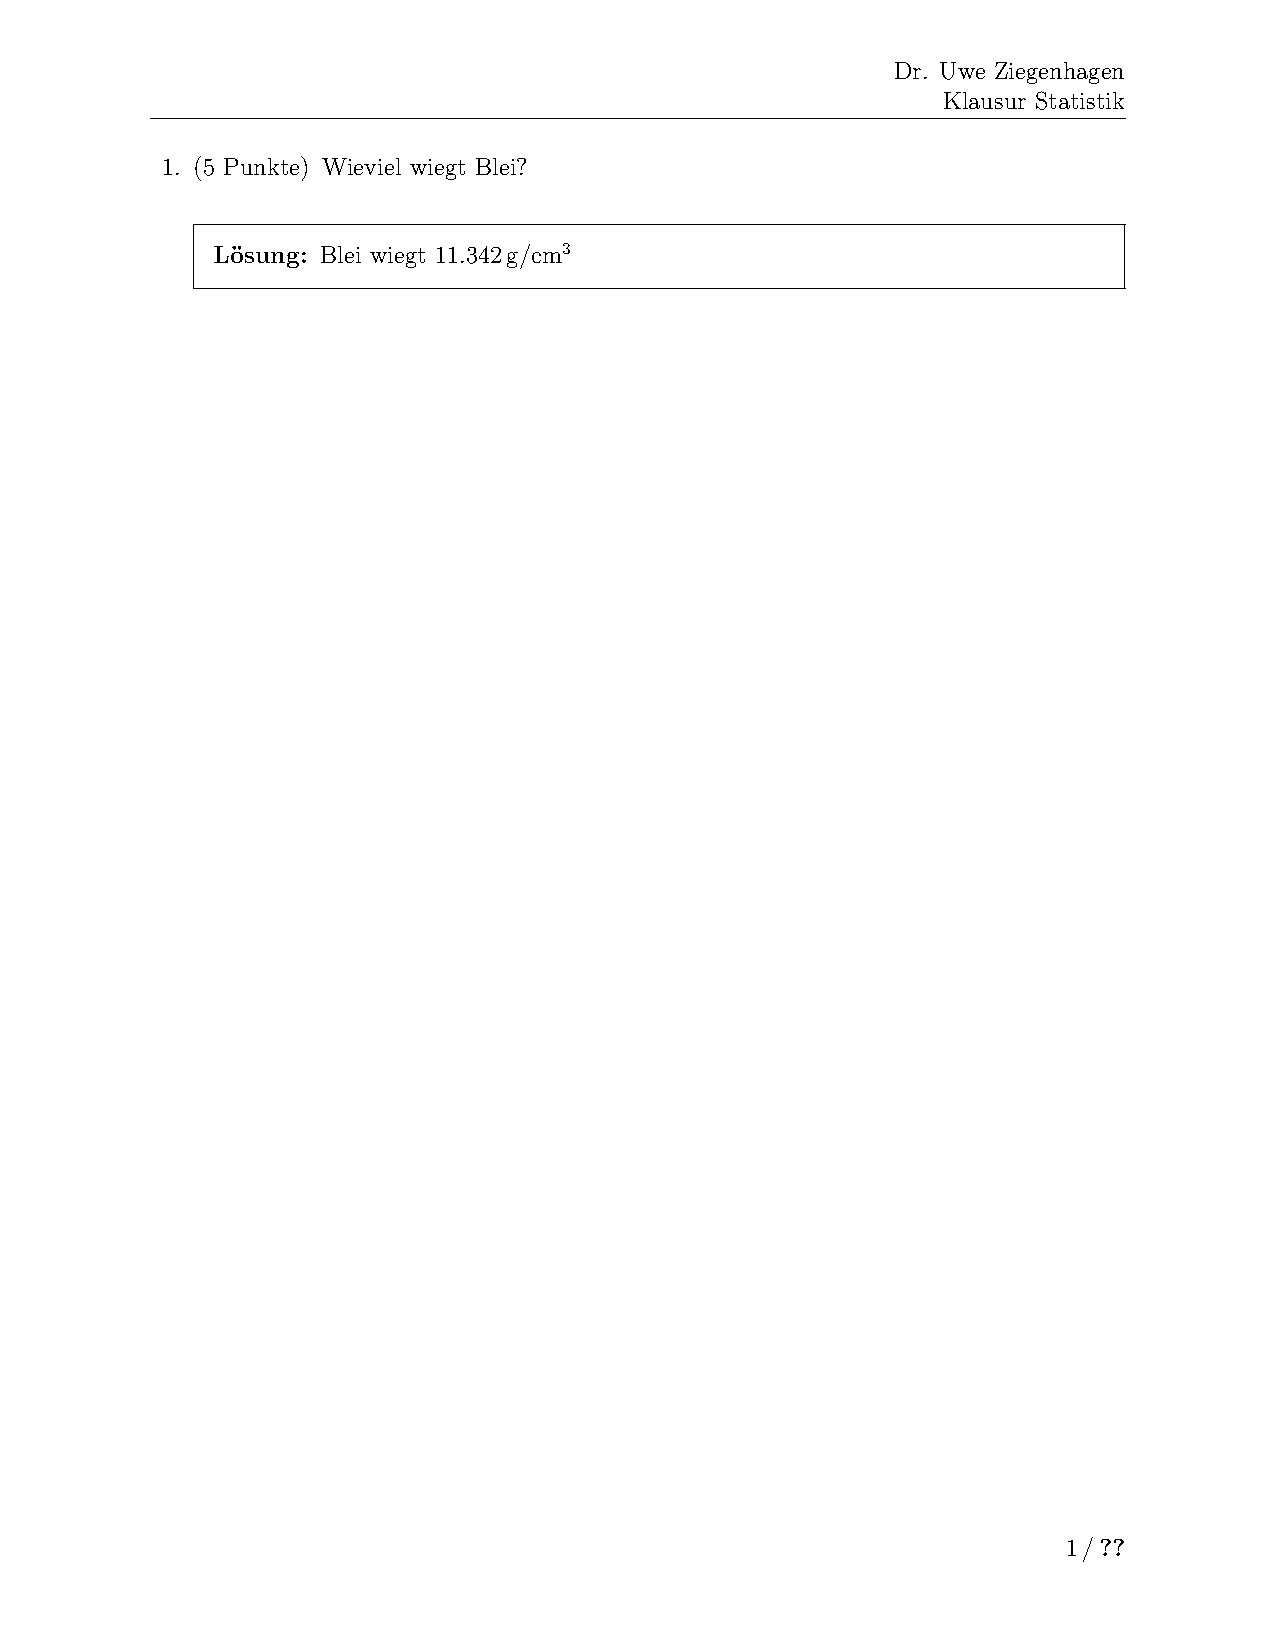
\includegraphics[clip, trim=2cm 22.5cm 2cm 0.7cm,width=\textwidth]{./Examples/exam/beispiel-10}} % 
\caption{Beispiel für die \texttt{solution} Umgebung}\label{fig:sol2}
\end{figure}

Alternativ biete das \texttt{exam} Paket auch die Möglichkeit, je nach gesetzter \enquote{answers} Option entweder die hinterlegte Lösung oder den Platz für die Antworten zu hinterlegen. Dazu stellt \texttt{exam} die folgenden Umgebungen bereit, deren jeweilige Bedeutung sich leicht aus dem Namen erschließt:

\begin{itemize}
	\item solutionorbox
	\item solutionorlines
	\item solutionordottedlines
	\item solutionorgrid
\end{itemize}

Die Abbildungen \ref{fig:solbox1} und \ref{fig:solbox2} zeigen am Beispiel von \texttt{solutionorgrid}, wie dies aussehen kann. Abbildung \ref{fig:solbox1} zeigt ein Gitter an, in das die Schüler die Lösung zeichnen können, Abbildung \ref{fig:solbox2} die Version mit Lösung\footnote{Für den Plot siehe \url{http://tex.stackexchange.com/questions/226277/how-to-plot-a-quadratic-equation-in-tikz}}.

\begin{figure}
\fbox{
\includegraphics[clip, trim=2cm 16.5cm 2cm 0.7cm,width=\textwidth]{./Examples/exam/beispiel-11}} % 
\caption{Ausgabe von \texttt{\textbackslash solutionorgrid} ohne gesetztes \enquote{answers}}\label{fig:solbox1}
\end{figure}

\begin{figure}
\fbox{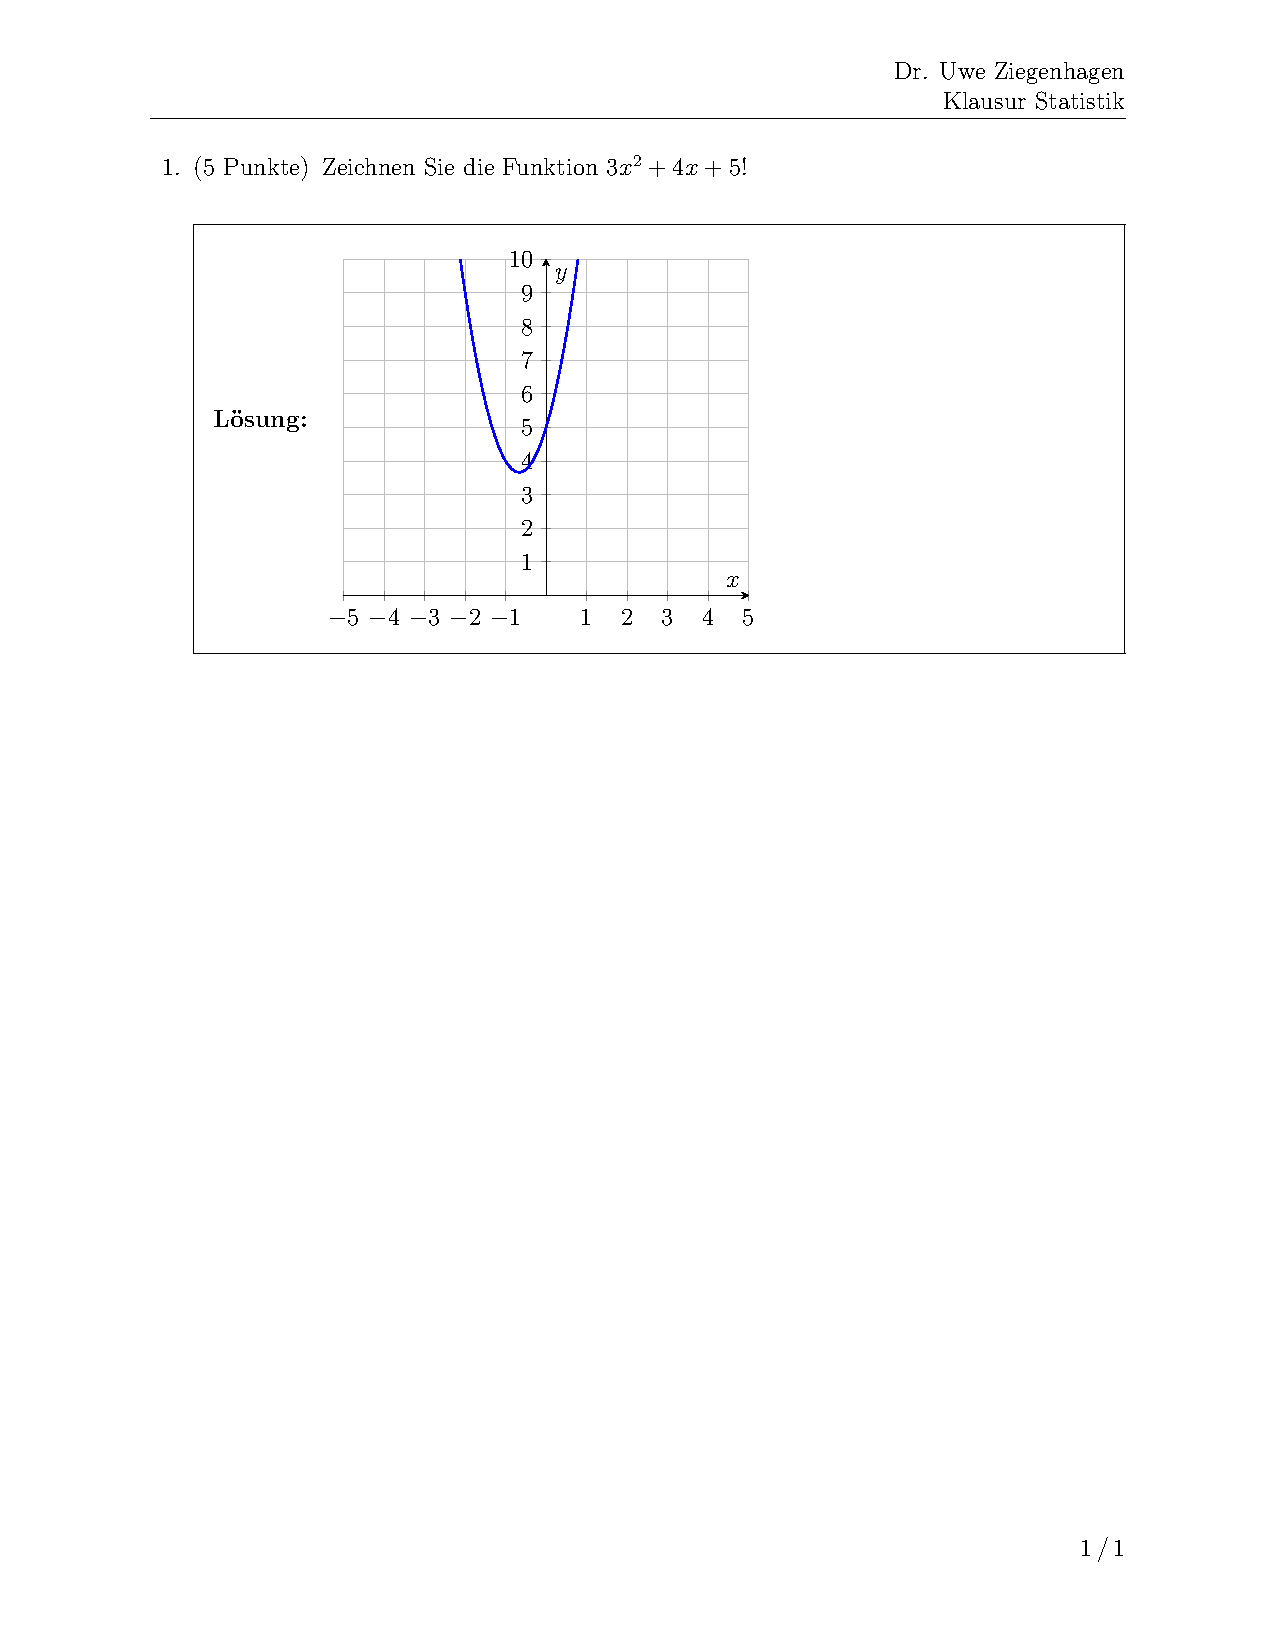
\includegraphics[clip, trim=2cm 15.5cm 2cm 0.7cm,width=\textwidth]{./Examples/exam/beispiel-12}} % 
\caption{Ausgabe von \texttt{\textbackslash solutionorgrid} mit gesetztem \enquote{answers}}\label{fig:solbox2}
\end{figure}


\section{Ausgabe von Notentabellen}

Wie bereits erwähnt kann \texttt{exam} auch Bewertungstabellen setzen, vertikal und horizontal, nach Aufgaben und nach Seiten. Listing \ref{lis:bew} zeigt die entsprechenden Befehle, die Abbildungen \ref{fig:hor} und \ref{fig:ver} zeigen jeweilige Ausgaben für horizontale Tabellen nach Fragen und Seiten.

\begin{lstlisting}[caption={Befehle für Bewertungstabellen},label={lis:bew}]
\gradetable[v][questions] vertikal nach Fragen
\gradetable[h][questions] horizontal nach Fragen
\gradetable[v][pages] vertikal nach Seiten
\gradetable[h][pages] horizontal nach Seiten
\end{lstlisting}

\begin{figure}[b]
\fbox{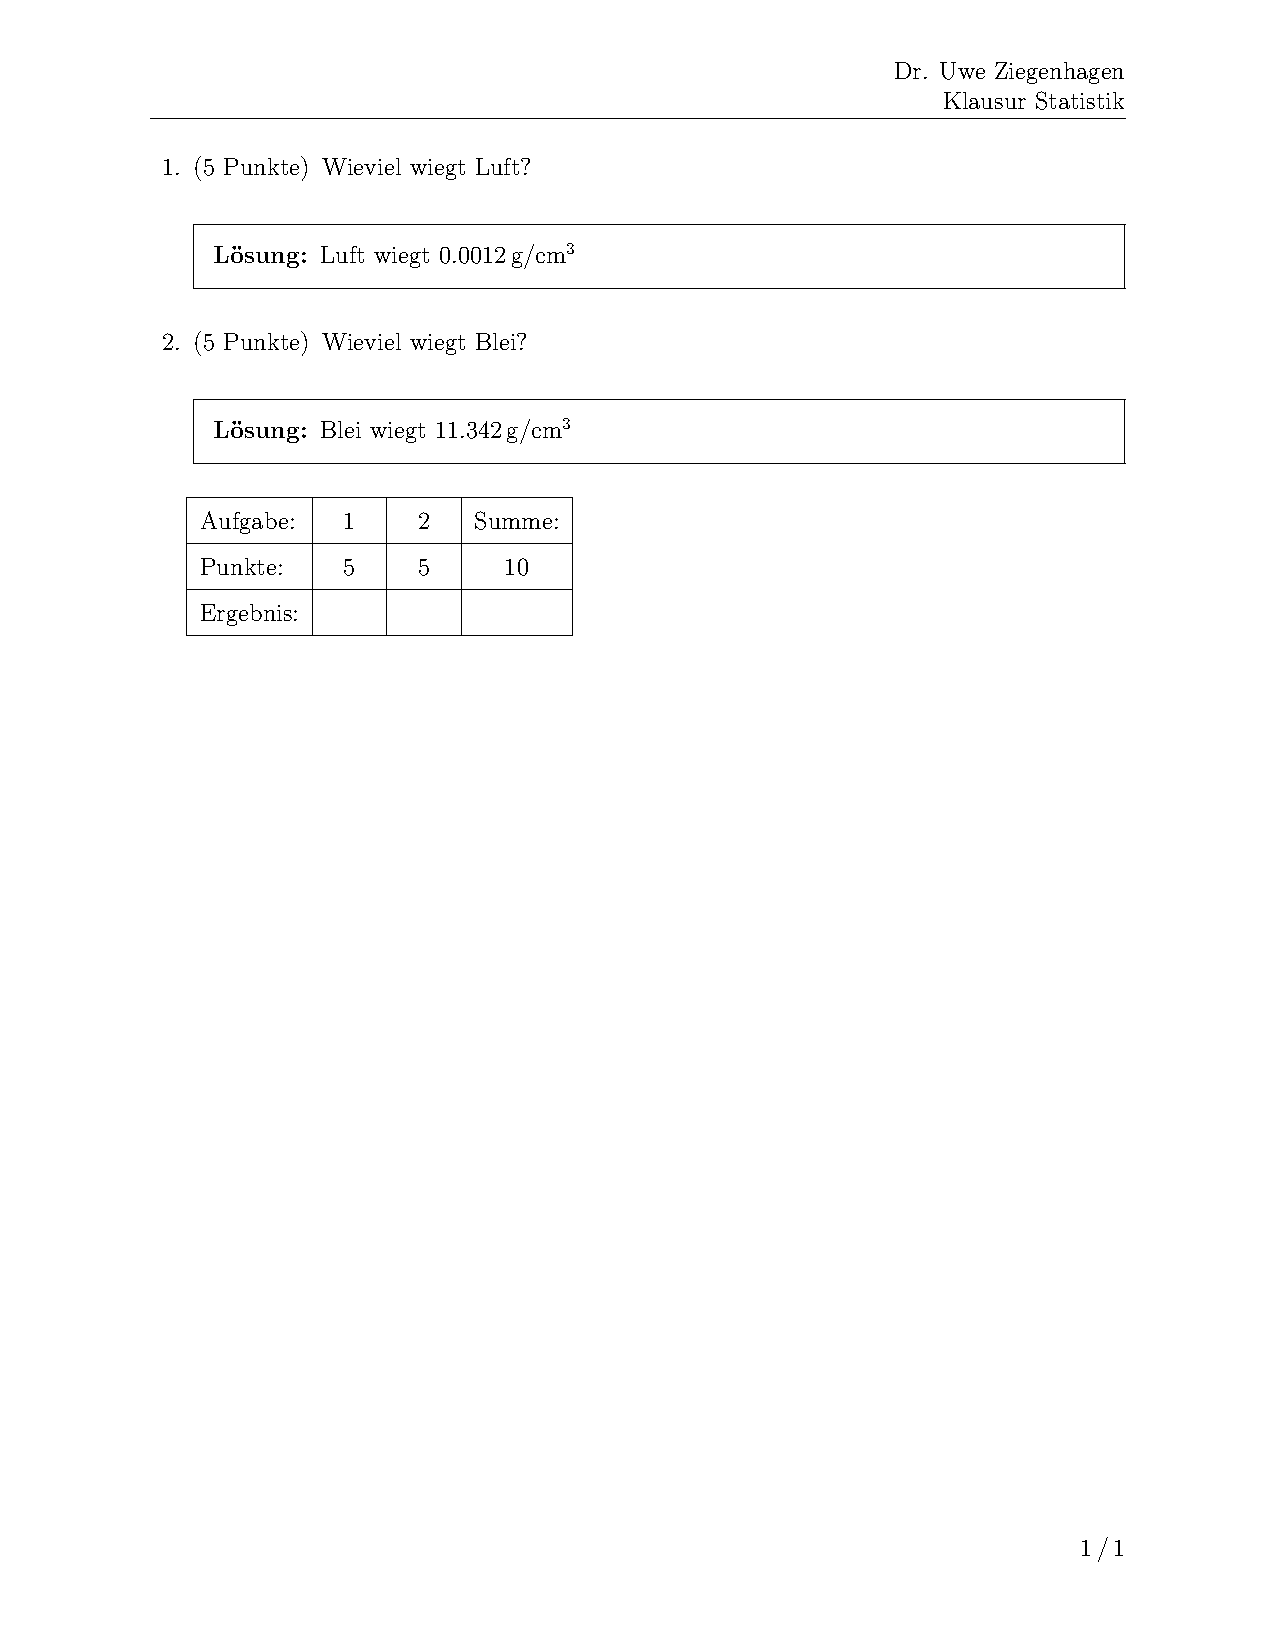
\includegraphics[clip, trim=2.5cm 15cm 2.5cm 0.7cm,width=\textwidth]{./Examples/exam/beispiel-13}} % 
\caption{Bewertungstabelle horizontal nach Fragen}\label{fig:hor}
\end{figure}

\begin{figure}
\fbox{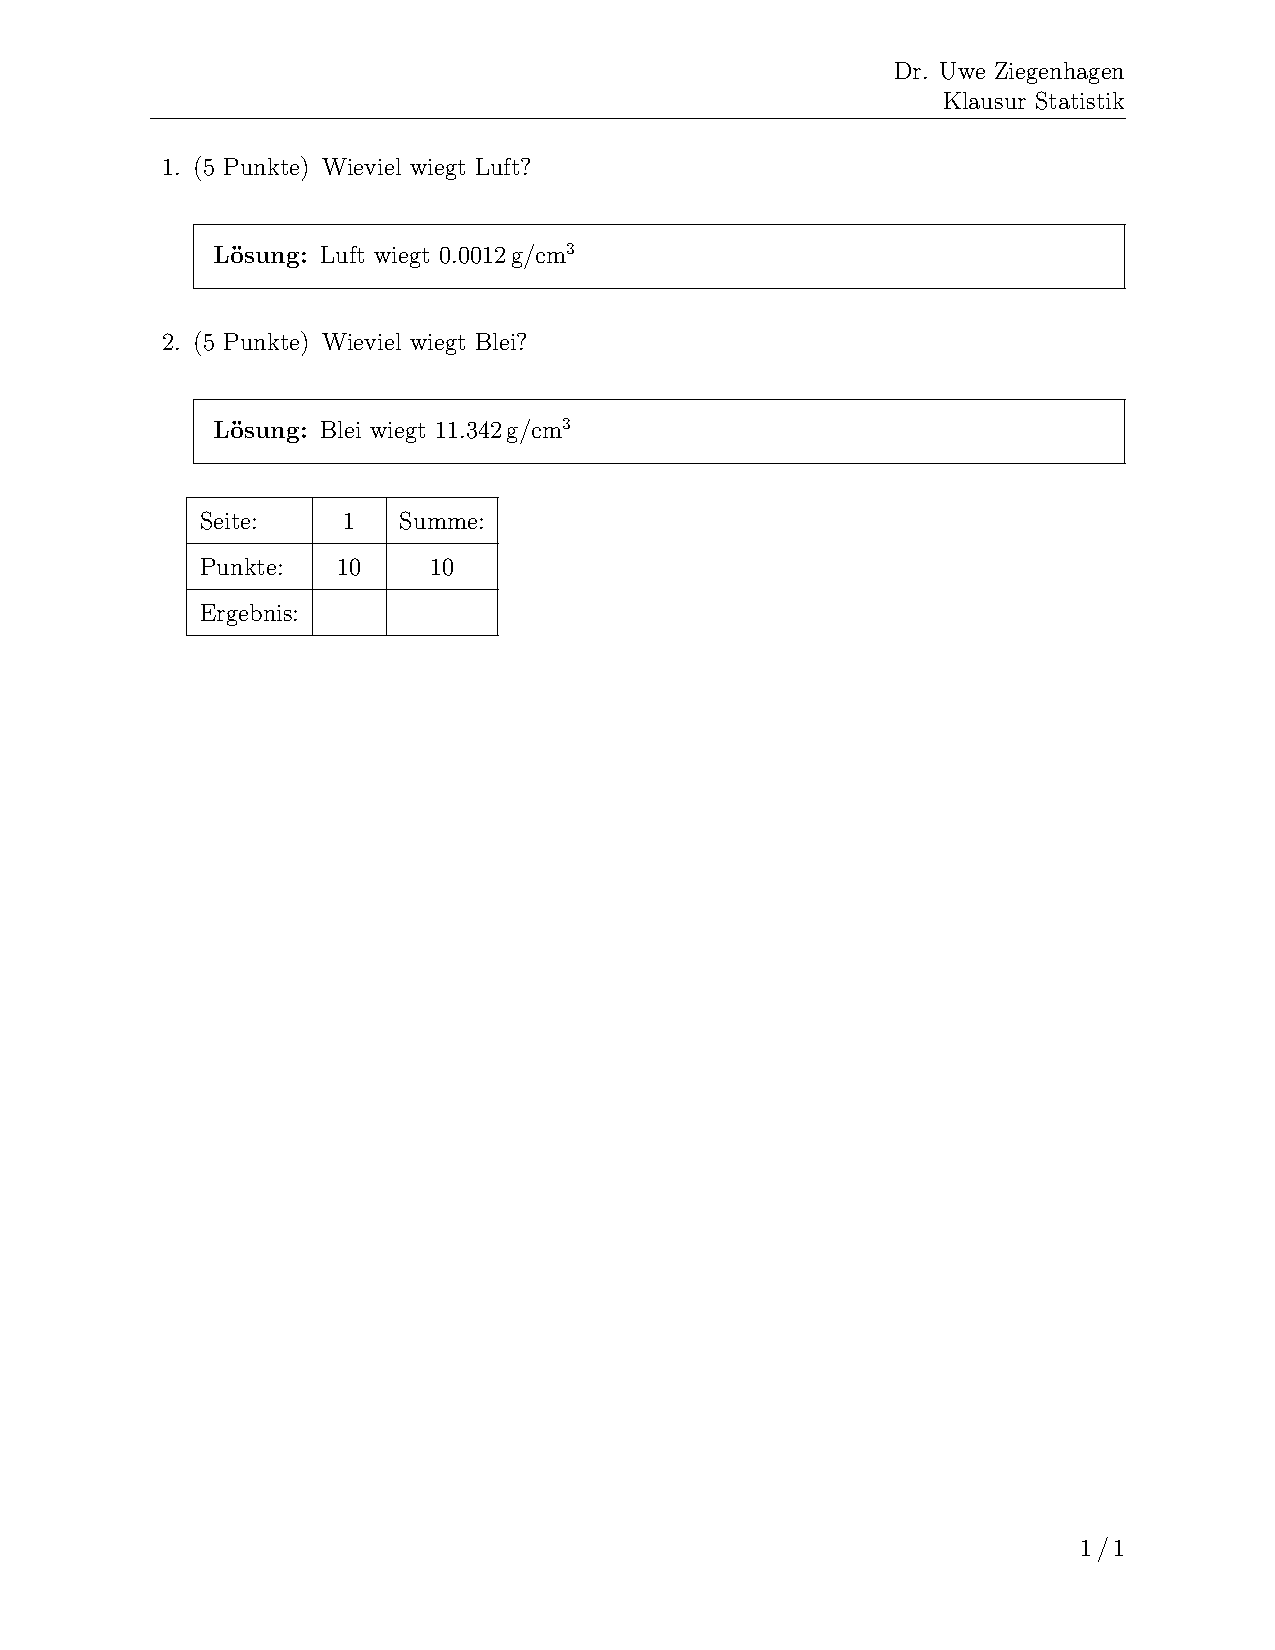
\includegraphics[clip, trim=2.5cm 17cm 2.5cm 0.7cm,width=\textwidth]{./Examples/exam/beispiel-14}} % 
\caption{Bewertungstabelle horizontal nach Seiten}\label{fig:ver}
\end{figure} 


\texttt{exam} bietet noch mehr, als diese kurze Einführung zeigen konnte, interessierten Lesern möchte ich daher nochmals die Dokumentation zum Paket empfehlen. 